\documentclass{article}

\usepackage[utf8]{inputenc}
\usepackage[T1]{fontenc}
\usepackage[greek,english]{babel}
\usepackage{alphabeta}
\usepackage{amsmath}
\usepackage{amssymb}
\usepackage{graphicx}
\usepackage{subcaption}
\usepackage{epstopdf}
\usepackage[margin=1in, paperwidth=7.5in,paperheight=10.5in]{geometry}
\usepackage{hyperref}
\usepackage{paracol}

\newcommand\course{ΗΡΥ 411}
\newcommand\courseName{Ενσωματωμένα Συστήματα Μικροεπεξεργατών}
\newcommand\semester{Χειμερινό 2020-2021}
\newcommand\assignmentNumber{Εργαστήριο 5}
\newcommand\studentName{Μαυρογιώργης Δημήτρης}                           
\newcommand\studentNumber{2016030016}

\title{\underline{\textbf{\assignmentNumber}}} 
\author{\textsc{\textbf{Όνομα:}}  \studentName\\
		\textsc{\textbf{ΑΜ:}}  \studentNumber\\
		\course \ - \courseName\\ 
		\textsc{Πολυτεχνείο Κρήτης}
		}
\date{\today}
\begin{document}
	\maketitle

\section*{Σκοπός}
	Σκοπός του τέταρτου εργαστηρίου είναι να μετατρεψουμε τo προηγούμενo εργαστήριο εξ' ολοκλήρου σε C, αλλά έχοντας υπόψη το τι ποροι χρησιμοποιούνται στον μικροελεγκτή AVR. Στόχος μας είναι δηλαδή να υλοποιήσουμε σε κώδικα C και τις συναρτήσεις για τα Interrupts των TIMER0 και USART, καθώς και όλων των βοηθητικών συναρτήσεων για clear της μνήμης και shift των αριθμών που αποθηκεύουμε σε ένα array κατά το receive. \\

\section*{Περιγραφή της υλοποίησης}
	Αρχικά, όσον αφορά το κωμάτι της μνήμης, οπως και στα προηγούμενα εργαστήρια με τη συνάρτηση MEM\_CLEAR αρχικοποιούμε τις θέσεις μνήμης που είναι αποθηκευμένοι οι αριθμοί με την τιμή "0x0A". Για το MEM\_SHIFT αυτό που κάνουμε έιναι ένα shift προς τα δεξιά όλων των στοιχείων του array.\\
	
	\noindent
	Παράλληλα, για τη ληψη και αποστολή μηνυμάτων δημιουργήθηκαν δύο συναρτήσεις, η USART\_RECEIVE και η USART\_TRANSMIT. Στην πρώτη, αυτό που γίνεται είναι να διαβάζουμε από τον καταχωρητή R15 και να επιστρέφουμε το αποτέλεσμα που διαβάστηκε. Οσον αφορά τη δεύτερη, αυτό που κάνουμε είναι να προσπαθούμε με polling να στείλουμε το μηνυμα OK<CR><LF>.\\
	
	\noindent
	Οσον αφορά τον TIMER0 OVF Handler αυτό που κάνουμε είναι να ελέγχουμε το digit counter για το ποιο ψηφιο προβάλλουμε στα 7-segments και αν η τιμη του έχει φτάσει το 0x08 σημαίνει ότι πρεπει να ξεκινήσουμε από το πρώτο στοιχείο. Στη συνέχεια, παίρνουμε από το array RECEIVED\_NUMBERS το στοιχείο στη θέση digit\_cnt. Παράλληλα, βγαζουμε στο PORTC έναν "1"στη θέση digit\_cnt. Στο PORTA βγάζουμε ως έξοδο το στοιχείο στη θέση display\_num, στην οποία βρίσκεται η αποκωδικοποίηση του αριθμού BCD που διαβάσαμε στη συγκεκριμένη μεταβλητή display\_num. Τέλος, αρχικοποιούμε τον καταχωρητή TCNT0 ξανά με την τιμή "0x63" και αυξάνουμε τον digit\_cnt κατα ένα.\\
	
	\pagebreak
	\noindent   
	Για τον Interrupt Handler του USART RXC αυτό που γίνεται είναι να διαβάζουμε τον καταχωρητή R15 με τη συνάρτηση USART\_RECEIVE και ελέγχουμε κάθε φορά τον τρέχοντα χαρακτήρα που λήφθηκε με τον προηγούμενο που αποθηκεύσαμε στη μνήμη. Αυτό γίνεται με σκοπό να ελέγχουμε αν έρχεται σωστά η εντολή και αναλόγως να κάνουμε την κατάλληλη ενέργεια και να στείλουμε το OK<CR><LF>, αν όλα έγιναν με επιτυχία. \\
	
	\begin{figure}[h!]
		\centering
		\begin{subfigure}[t]{0.5\textwidth}
			\centering
			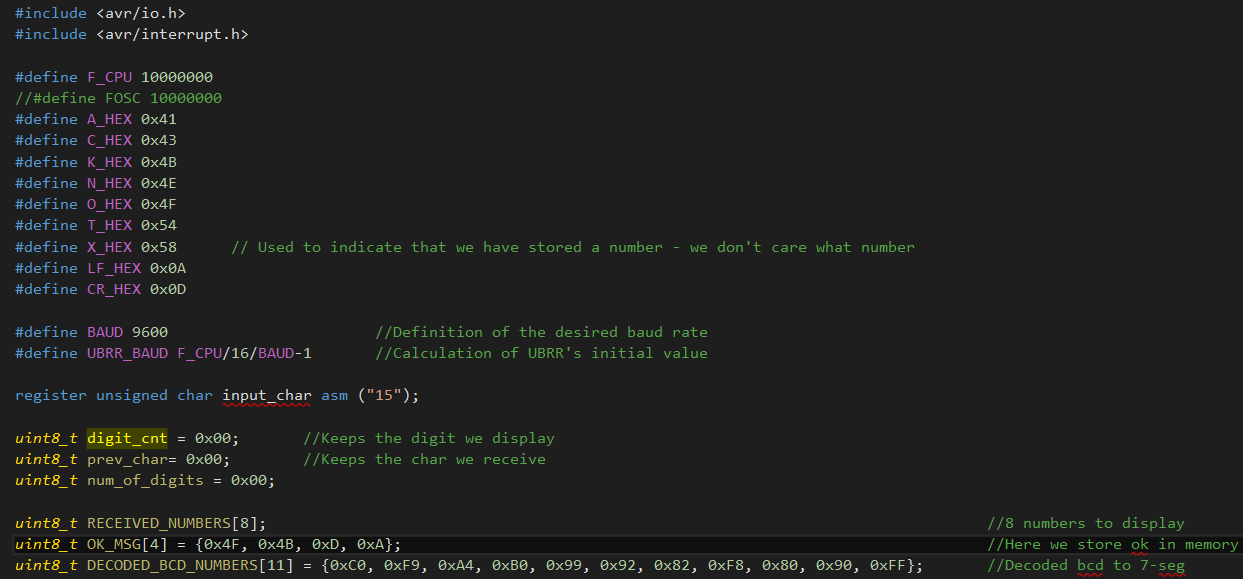
\includegraphics[height=3.5cm, width=\linewidth]{./results/lab5_defines.png}
			\caption{C code for define global variables}
		\end{subfigure}%
		~
		\begin{subfigure}[t]{0.5\textwidth}
			\centering
			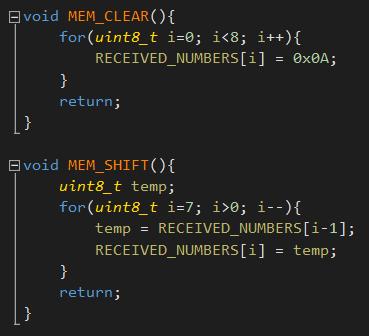
\includegraphics[height=3.5cm, width=\linewidth]{./results/lab5_mem_handling.png}
			\caption{C code for memory clear and shift}
		\end{subfigure}
	
		\begin{subfigure}[t]{0.5\textwidth}
			\centering
			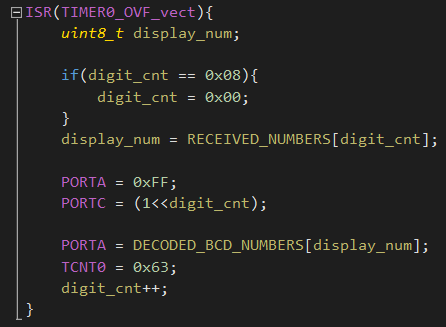
\includegraphics[height=3.5cm, width=\linewidth]{./results/lab5_timer0_handler.png}
			\caption{C code for TIMER0 OVF Interrupt Handler}
		\end{subfigure}%
		~
		\begin{subfigure}[t]{0.5\textwidth}
			\centering
			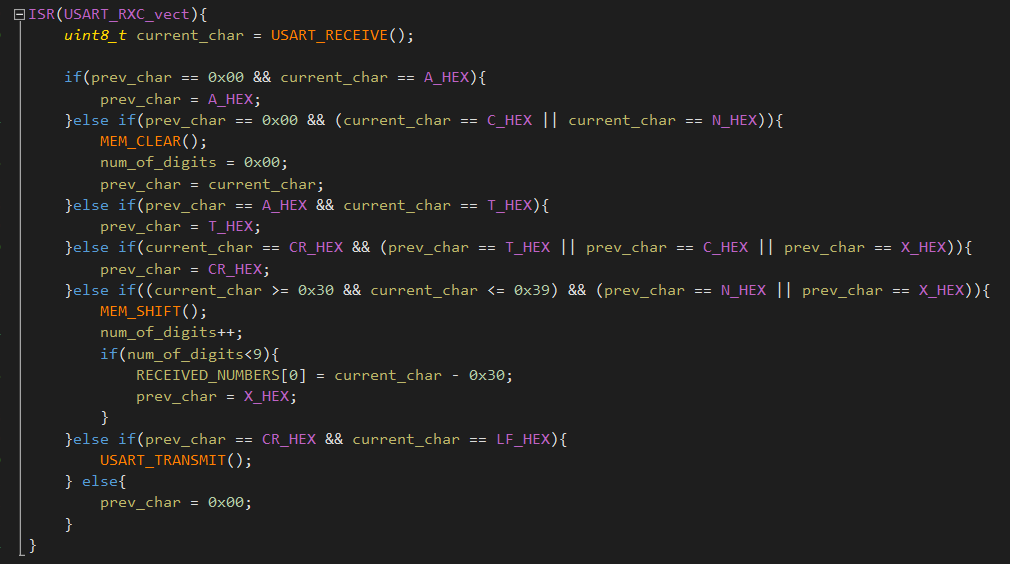
\includegraphics[height=3.5cm, width=\linewidth]{./results/lab5_usart_handler.png}
			\caption{C code for USART RXC Interrupt Handler}
		\end{subfigure}	
	
		\begin{subfigure}[t]{0.5\textwidth}
			\centering
			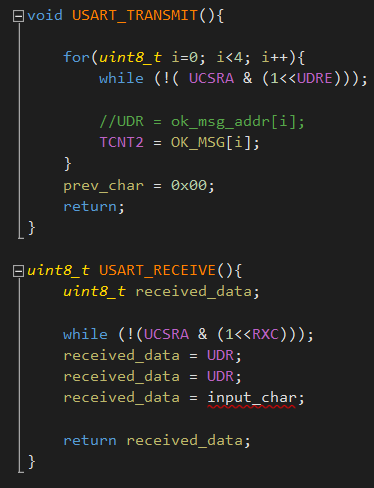
\includegraphics[height=3.5cm, width=\linewidth]{./results/lab5_usart_receive_transmit.png}
			\caption{C code for USART transmit and receive}
		\end{subfigure}	
	\end{figure}

	\noindent
	\textbf{Προσομοίωση Αποτελεσμάτων} \\
	
	\noindent
	Οι προσομοιώσεις του συγκεκριμένου εργαστηρίου είναι ακριβώς ίδιες με των προηγούμενων, εφόσον δεν προστέθηκαν επιπλέον λειτουργίες. Eιδικότερα, στις παρακάτω εικόνες φαίνεται ότι γίνεται σωστά το initialization των καταχωρητών του TIMER0 και USART, καθώς και η αποθήκευση των αποκωδικοποιήσεων για τα 7-segment και του μηνυματος OK<CR><LF>. Παρατηρούμε ότι όλες οι τιμές αποθηκεύονται σειριακά στη μνήμη ξεκινώντας από τη διεύθυνση "0x60". Eπίσης, βλέπουμε ότι εκτελείται σωστά ο USART handler και οι τιμές οι οποίες λαμβάννται αποθηκεύονται στη μνήμη, ενώ τέλος φαίνεται ότι εκτελείται σωστά και ο TIMER0 handler και γίνεται σωστά η ανανέωση των ψηφίων των 7-segments κάθε περίπου 1 ms.
	\pagebreak
	\begin{figure}[h!]
		\centering
		\begin{subfigure}[t]{0.5\textwidth}
			\centering
			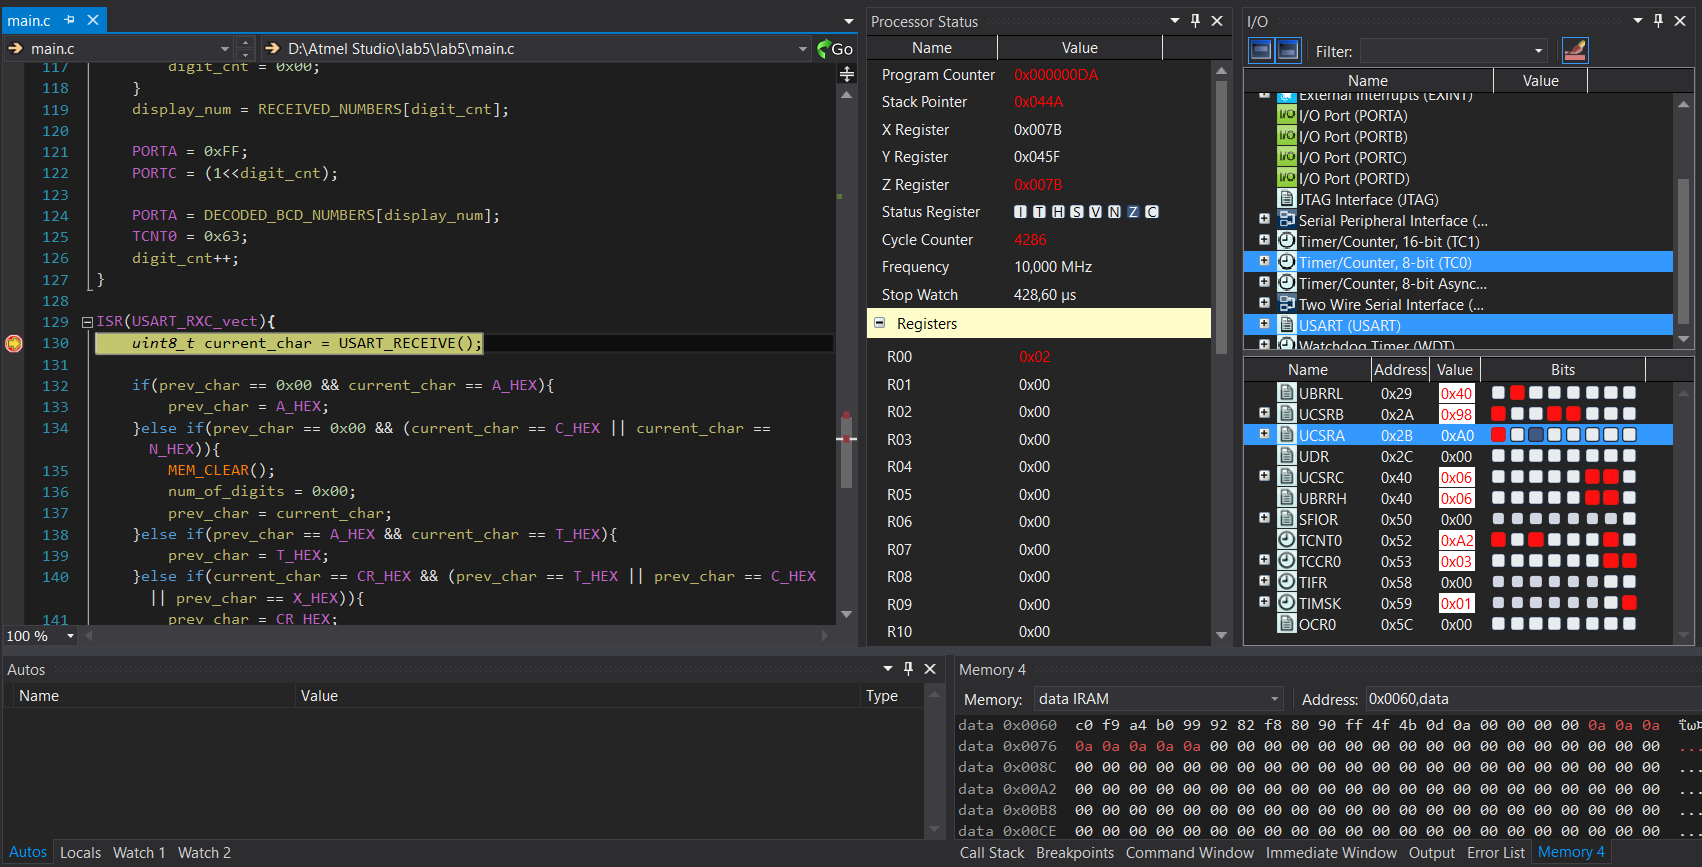
\includegraphics[height=3.5cm, width=\linewidth]{./results/lab5_sim_init.png}
			\caption{Αtmel Studio 7 - Initialization of TIMER0 and USART}
		\end{subfigure}%
		~
		\begin{subfigure}[t]{0.5\textwidth}
			\centering
			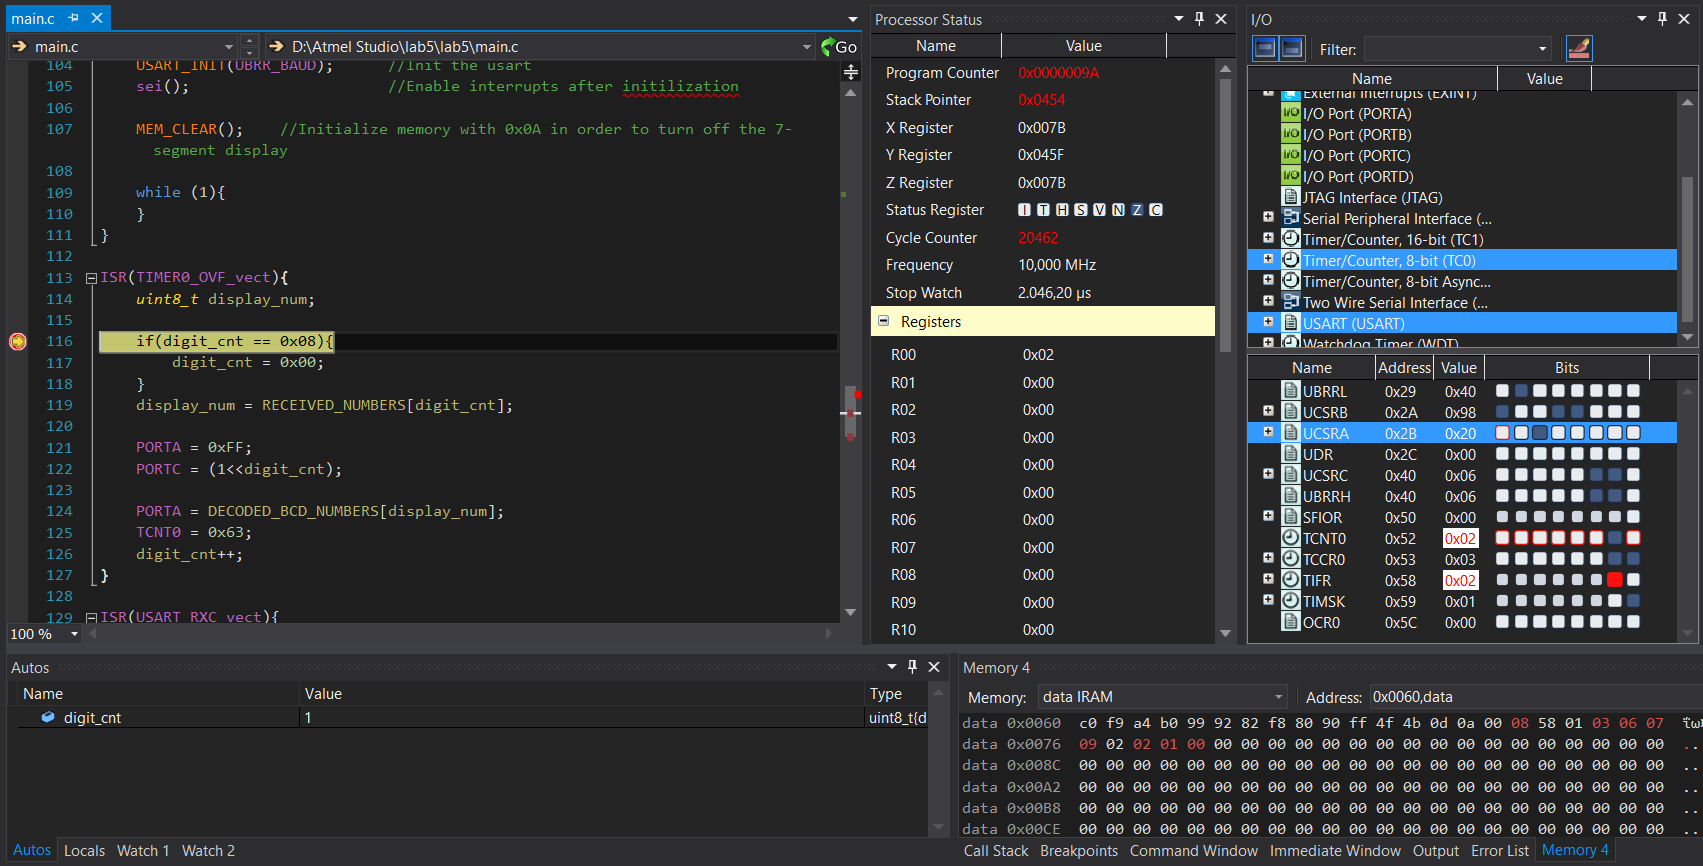
\includegraphics[height=3.5cm, width=\linewidth]{./results/lab5_sim_num_instruction.png}
			\caption{Αtmel Studio 7 - Execution of N01229763<CR><LF>}
		\end{subfigure}
		
		\begin{subfigure}[t]{0.5\textwidth}
			\centering
			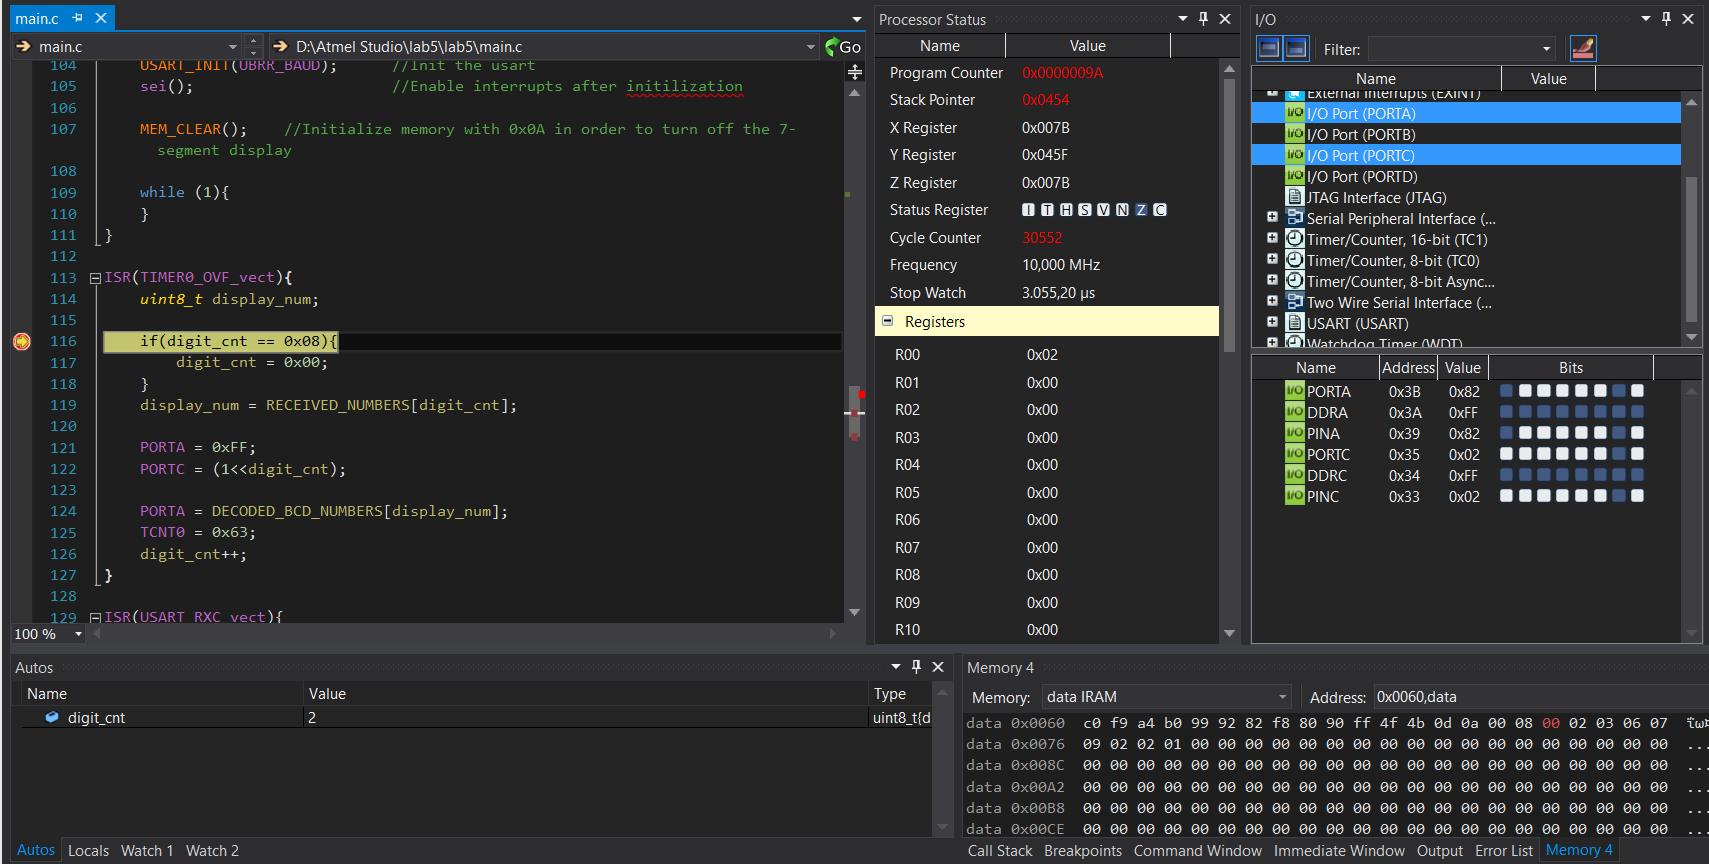
\includegraphics[height=3.5cm, width=\linewidth]{./results/lab5_sim_timer0_digit1.png}
			\caption{Αtmel Studio 7 - Display Digit 1}
		\end{subfigure}%
		~
		\begin{subfigure}[t]{0.5\textwidth}
			\centering
			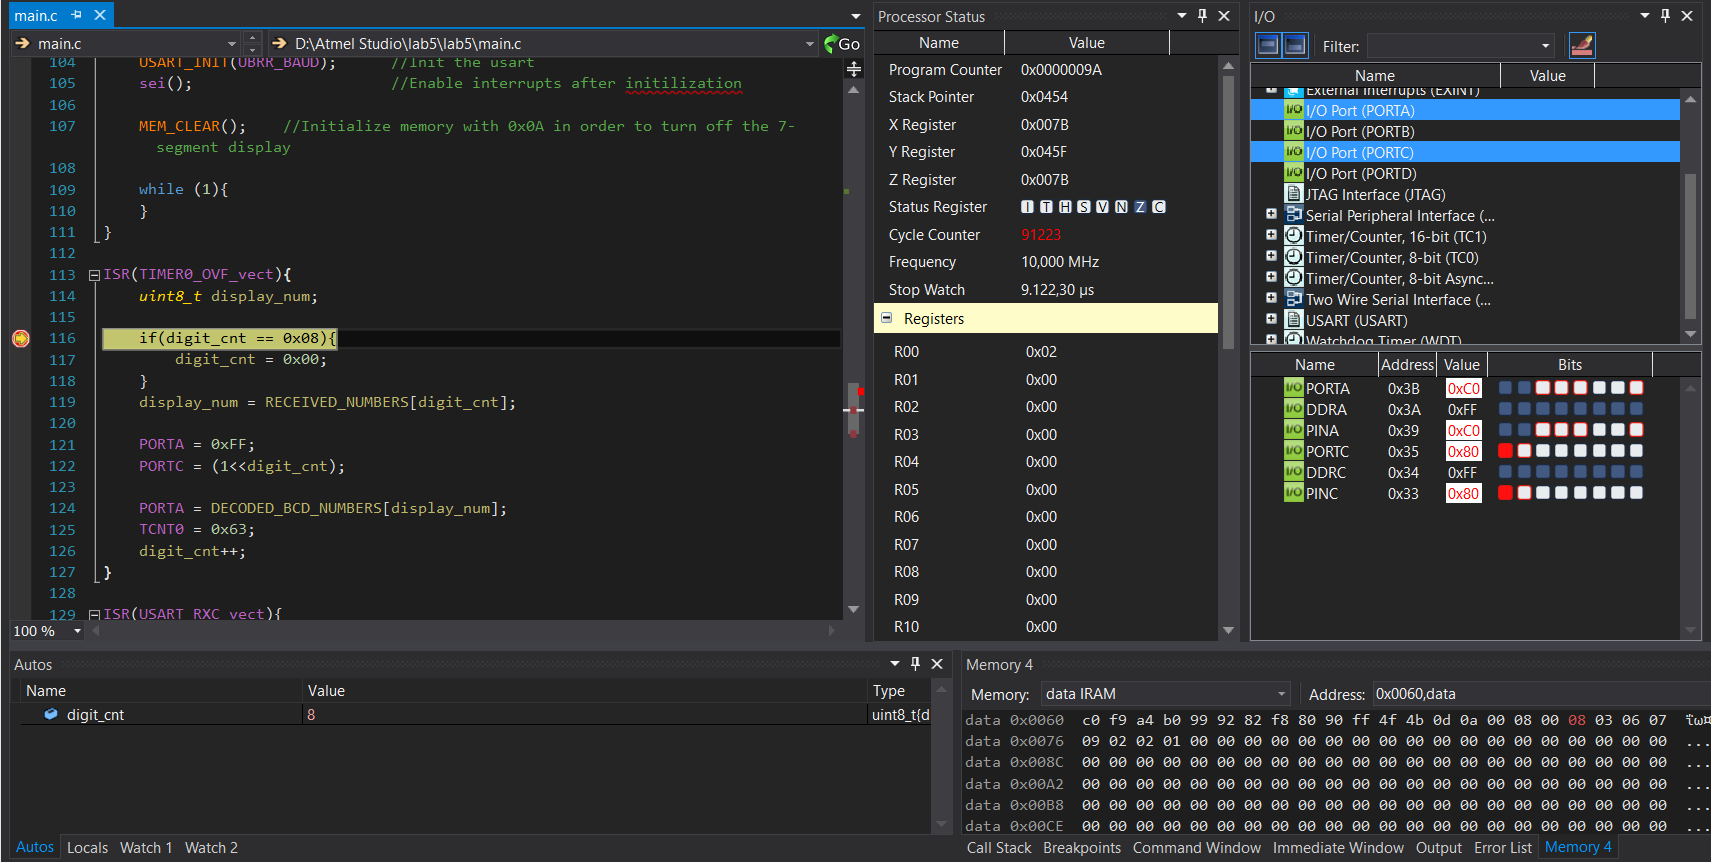
\includegraphics[height=3.5cm, width=\linewidth]{./results/lab5_sim_timer0_digit7.png}
			\caption{Αtmel Studio 7 - Display Digit 7}
		\end{subfigure}	
	\end{figure}	
\end{document}
